% =============================================================
%  Feature-engineering brainstorm for Transavia
%  Author: Noah Bos
%  Purpose: structure tomorrow's brainstorm on candidate predictors
%  Style: Accenture-inspired (purple #A100FF, sans-serif, clean)
%  Compile: pdflatex feature_brainstorm_transavia.tex   (run twice)
% =============================================================

\documentclass[aspectratio=169,11pt]{beamer}

% ---- Packages ----
\usepackage[T1]{fontenc}
\usepackage[utf8]{inputenc}
\usepackage{lmodern}
\usepackage{helvet}
\renewcommand{\familydefault}{\sfdefault}
\usepackage{xcolor}
\usepackage{tikz}
\usetikzlibrary{positioning, arrows.meta}
\usepackage{booktabs}
\usepackage{array}
\usepackage{tabularx}
\usepackage{calc}

% ---- Accenture palette ----
\definecolor{accpurple}{HTML}{A100FF}
\definecolor{accdark}{HTML}{1F1F1F}
\definecolor{accgray}{HTML}{6B6B6B}
\definecolor{accbg}{HTML}{F5F2FA}
\definecolor{accaccent}{HTML}{460073}
\definecolor{accgreen}{HTML}{1AAF54}
\definecolor{accred}{HTML}{D6336C}

% ---- Beamer setup ----
\setbeamertemplate{navigation symbols}{}
\setbeamertemplate{footline}{%
  \leavevmode%
  \hbox{%
    \begin{beamercolorbox}[wd=\paperwidth, ht=2.5ex, dp=1ex, right, rightskip=1.2em]{}%
      \color{accpurple}\scriptsize\insertframenumber{}\,/\,\inserttotalframenumber
    \end{beamercolorbox}}\vskip0pt%
}

\setbeamercolor{frametitle}{fg=accdark, bg=white}
\setbeamercolor{title}{fg=accdark}
\setbeamercolor{normal text}{fg=accdark, bg=white}
\setbeamercolor{itemize item}{fg=accpurple}
\setbeamercolor{itemize subitem}{fg=accpurple}
\setbeamercolor{itemize subsubitem}{fg=accpurple}
\setbeamercolor{enumerate item}{fg=accpurple}
\setbeamercolor{block title}{fg=white, bg=accpurple}
\setbeamercolor{block body}{fg=accdark, bg=accbg}
\setbeamercolor{alerted text}{fg=accred}

\setbeamerfont{frametitle}{size=\large, series=\bfseries}
\setbeamerfont{title}{size=\LARGE, series=\bfseries}
\setbeamerfont{subtitle}{size=\normalsize, series=\mdseries}

\setbeamertemplate{frametitle}{%
  \vspace{0.8em}%
  \hspace{0.6em}\insertframetitle\\[-0.2em]%
  \hspace{0.6em}\textcolor{accpurple}{\rule{2.5em}{2pt}}\vspace{0.4em}%
}

\setbeamertemplate{itemize item}{\raisebox{0.3ex}{\scalebox{0.7}{\textcolor{accpurple}{$\blacksquare$}}}}
\setbeamertemplate{itemize subitem}{\raisebox{0.3ex}{\scalebox{0.6}{\textcolor{accpurple}{$\blacktriangleright$}}}}

% Title page template
\defbeamertemplate*{title page}{accenture}{%
  \begin{tikzpicture}[remember picture, overlay]
    \fill[accpurple] (current page.north west) rectangle ([yshift=-1.3cm]current page.north east);
    \fill[accaccent] ([yshift=-1.3cm]current page.north west) rectangle ([yshift=-1.45cm]current page.north east);
  \end{tikzpicture}%
  \vspace{2.8cm}
  \begin{flushleft}
    \hspace{0.8em}{\color{accpurple}\rule{3em}{3pt}}\\[0.6em]
    \hspace{0.8em}{\usebeamerfont{title}\inserttitle}\\[0.4em]
    \hspace{0.8em}{\color{accgray}\usebeamerfont{subtitle}\insertsubtitle}\\[1.6em]
    \hspace{0.8em}{\color{accdark}\small\insertauthor}\\[0.2em]
    \hspace{0.8em}{\color{accgray}\footnotesize\insertdate}
  \end{flushleft}
}

% Coloured chips
\newcommand{\chip}[2]{\tikz[baseline=(c.base)]{\node[fill=#1!15, draw=#1, line width=0.4pt, rounded corners=2pt, inner sep=2pt, text=#1, font=\scriptsize\bfseries] (c) {#2};}}
\newcommand{\good}[1]{\chip{accgreen}{#1}}
\newcommand{\warn}[1]{\chip{accred}{#1}}
\newcommand{\info}[1]{\chip{accpurple}{#1}}
\newcommand{\tierA}[0]{\chip{accgreen}{Tier A}}
\newcommand{\tierB}[0]{\chip{accpurple}{Tier B}}

% =============================================================
%  TITLE
% =============================================================
\title{Brainstorming new predictors for luggage CTR}
\subtitle{To kickstart, I dug into L5B15 \textemdash{} let's react to it together}
\author{Noah Bos \textbar{} Accenture \textbar{} Leiden University thesis}
\date{June 2026}

\begin{document}

% ---------- Title ----------
\begin{frame}[plain, noframenumbering]
  \titlepage
\end{frame}

% =============================================================
%  FRAME 2 — Framing
% =============================================================
\begin{frame}{Starting point: today L5B15 is mostly a \emph{fatigue machine}}
  \footnotesize
  Healthy NB model (AUC \(\approx 76.6\)), but the 23 active predictors lean one way:
  \begin{itemize}
    \setlength\itemsep{0em}
    \item \textbf{11 Interaction History counters} \textemdash{} all Email or Push, mostly Pending
    \item \textbf{11 booking-context fields} \textemdash{} mostly flight metadata
    \item \textbf{1 strategy parameter} (\emph{BundleName})
    \item \textbf{0 Customer attributes active} (220+ configured, none picked up)
  \end{itemize}
  \vspace{0.5em}
  \begin{block}{So what drives the score is mostly recency / volume}
    \footnotesize Almost nothing about the customer or the trip itself. \textbf{That's the headroom we want to brainstorm into.}
  \end{block}
\end{frame}

% =============================================================
%  FRAME 3 — Today's top 10 (SHAP)
% =============================================================
\begin{frame}{What the model leans on most today}
  \vspace{-0.6em}
  {\scriptsize Top 15 active features by mean \(|\)SHAP\(|\) on L5B15, coloured by category:}
  \vspace{-0.4em}
  \begin{center}
    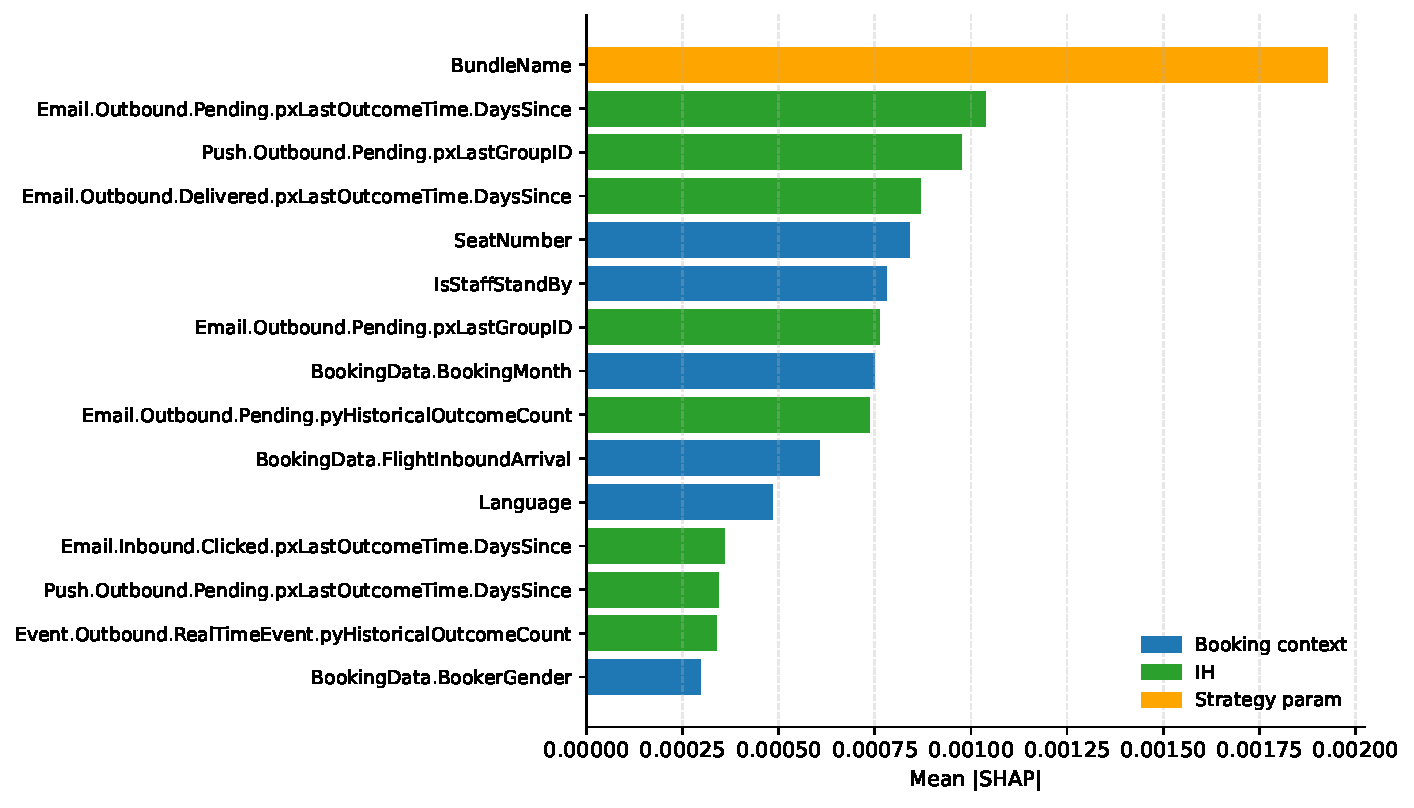
\includegraphics[height=0.66\textheight,keepaspectratio]{figures/shap_top15_l5b15_by_category.pdf}
  \end{center}
  \vspace{-0.6em}
  {\scriptsize Green = recency / volume of past contact; blue = flight-context; orange = strategy parameter. \emph{No customer-level field is in the list.}}
\end{frame}

% =============================================================
%  FRAME 4 — What's in Pega but unused
% =============================================================
\begin{frame}{First, what's already inside Pega that the model isn't using?}
  \vspace{-0.3em}
  \footnotesize
  Pega's \texttt{pdstools} has a notebook that ranks \emph{every} field already flowing into the model, not just the 23 NB picked. I ran it on L5B15 ahead of time so we have something to react to. Top candidates currently sitting outside the active set:
  \vspace{0.2em}
  \scriptsize
  \renewcommand{\arraystretch}{0.95}
  \begin{tabular}{@{}p{0.34\linewidth} r p{0.50\linewidth}@{}}
    \toprule
    \textbf{Candidate} & \textbf{Imp.} & \textbf{Why it might matter} \\
    \midrule
    Booking create date-time          & 0.109 & \warn{caveat}: likely a timing leak; needs validation \\
    Email-out Delivered, hist.\ count & 0.042 & how often Pega \emph{tries} to email this customer \\
    Booker language                   & 0.025 & customer-side, not just flight-context language \\
    Booker role on booking            & 0.022 & primary booker vs.\ travel companion \\
    Days booking-to-flight            & 0.020 & last-minute vs.\ planned travel \\
    Email-in Clicked, last group ID   & 0.020 & most recent \emph{inbound} engagement context \\
    Branded fare bought               & 0.019 & Basic / Plus / Max \(\to\) willingness to pay \\
    \bottomrule
  \end{tabular}
  \vspace{0.3em}
  \normalsize
  \begin{block}{One thing worth flagging}
    \footnotesize Many \emph{customer-level} fields are 75\,\%+ missing on L5B15. NB drops them as a result \textemdash{} so the gap isn't that they're bad predictors, it's that the data isn't flowing. Re-enabling these is usually the lighter lift.
  \end{block}
\end{frame}

% =============================================================
%  FRAME 4 — Tier B canvas
% =============================================================
\begin{frame}{Then \textemdash{} what could we bring in from outside Pega?}
  \vspace{-0.3em}
  \footnotesize
  Some guesses to get the conversation going. Left = why we might expect a lift; right = roughly where the data would have to live.
  \vspace{0.2em}
  \scriptsize
  \renewcommand{\arraystretch}{1.05}
  \begin{tabular}{@{}p{0.20\linewidth} p{0.40\linewidth} p{0.34\linewidth}@{}}
    \toprule
    \textbf{Why it might help} & \textbf{What we'd add} & \textbf{Where it would come from} \\
    \midrule
    Personalisation
      & Per-product purchase history (luggage, seats, meals, priority)
      & Already configured as \texttt{CustomerKPIs.*} but mostly missing \\[0.2em]
    Trip purpose
      & Duration \(\times\) destination type \(\times\) children-on-PNR \(\times\) weekday
      & Party composition; a destination-type lookup \\[0.2em]
    Route economics
      & Route type (leisure vs.\ business); avg luggage attach rate per route
      & Aggregate attach rate by route, last few months \\[0.2em]
    Price sensitivity
      & Discount redemptions; ancillary added \emph{after} booking vs.\ at booking
      & Booking-modification log, timestamped, on PNR \\[0.2em]
    Context
      & Weather / season at destination on the flight date
      & A weather table keyed on IATA + date \\[0.2em]
    Loyalty
      & Tier, months since first booking, distinct destinations flown
      & Customer master with tier history \\
    \bottomrule
  \end{tabular}
  \vspace{0.2em}
  \normalsize
  {\scriptsize\textcolor{accgray}{Just starting points \textemdash{} add, remove, replace.}}
\end{frame}

% =============================================================
%  FRAME 6 — Validation method
% =============================================================
\begin{frame}{How we'd actually test any of this}
  \vspace{-0.3em}
  \footnotesize
  The same Pega \texttt{pdstools} notebook works for both flavours \textemdash{} I can wire each candidate up so we just need to point it at the data:
  \vspace{0.3em}

  \begin{center}
  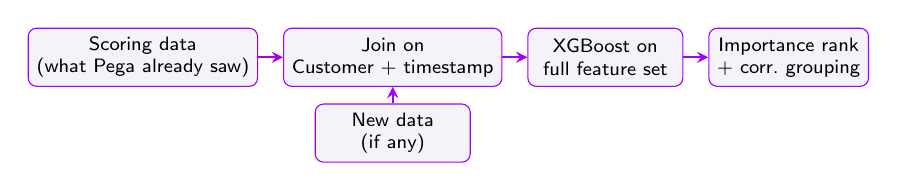
\begin{tikzpicture}[
    node distance=0.3em and 0.9em,
    box/.style={draw=accpurple, rounded corners=3pt, fill=accbg, font=\scriptsize, align=center, inner sep=3pt, minimum height=2.1em, minimum width=5.6em},
    arrow/.style={->, >=stealth, accpurple, thick}
  ]
    \node[box] (hds)    {Scoring data\\(what Pega already saw)};
    \node[box, right=of hds] (join) {Join on\\Customer + timestamp};
    \node[box, right=of join] (xgb)  {XGBoost on\\full feature set};
    \node[box, right=of xgb] (rank)  {Importance rank\\+ corr.\ grouping};
    \node[box, below=of join, yshift=-0.3em] (lake) {New data\\(if any)};
    \draw[arrow] (hds)  -- (join);
    \draw[arrow] (lake) -- (join);
    \draw[arrow] (join) -- (xgb);
    \draw[arrow] (xgb)  -- (rank);
  \end{tikzpicture}
  \end{center}

  \vspace{0.3em}
  \scriptsize
  \begin{itemize}
    \setlength\itemsep{0.1em}
    \item No leakage: each row picks the latest snapshot \emph{before} the decision was made
    \item Verdict per idea: (a) does it rank in the top-20? (b) is it redundant with something already active? (c) does it lift held-out AUC?
    \item Anything new from outside Pega just needs a Customer/PNR key and a timestamp
  \end{itemize}
  \vspace{0.3em}
  \normalsize
  {\scriptsize\textcolor{accgray}{Re-running on what's already in Pega is the easier lift; pulling in something new is more work, but that's also where the bigger upside likely sits.}}
\end{frame}

% =============================================================
%  FRAME 7 — Closing / discussion
% =============================================================
\begin{frame}{Still open}
  \footnotesize
  \begin{enumerate}
    \setlength\itemsep{0.7em}
    \item For the inactive fields on slide 4 \textemdash{} are any blocked by an upstream feed (Booker language, Branded fare, Days-to-flight), or is it just a config switch?
    \item \texttt{CustomerKPIs.*} is 75\,\%+ missing. Is Transavia not sourcing it, or is Pega not subscribed? Probably the biggest single unblock.
    \item Of the outside-Pega ideas on slide 5 \textemdash{} which already live as tables in the data lake, and which would need to be built?
    \item Separately: any appetite to also pilot Pega's \textbf{AGB} in shadow mode? That tells us whether the headroom is feature-side or model-side.
  \end{enumerate}
  \vspace{0.6em}
  {\scriptsize\textcolor{accgray}{Slides 3 \& 4 are L5B15 only \textemdash{} happy to run the same view on CLUG / BookingDotCom / Cartrawler if useful.}}
\end{frame}

% ---------- Closing ----------
\begin{frame}[plain, noframenumbering]
  \begin{tikzpicture}[remember picture, overlay]
    \fill[accpurple] (current page.south west) rectangle (current page.north east);
  \end{tikzpicture}
  \vfill
  \begin{center}
    \color{white}{\fontsize{34}{38}\selectfont\textbf{Over to you}}\\[1em]
    \color{white}{\rule{4em}{2pt}}\\[1em]
    \color{white}{\normalsize Noah Bos \textbar{} noah.bos@accenture.com}
  \end{center}
  \vfill
\end{frame}

\end{document}
